\section{Results and Discussion}
This chapter present the performance evaluation of various machine learning models for emotion classification and discuss their strengths and limitations. Six models—Naive Bayes, Logistic Regression, Random Forest, Support Vector Machine (SVM), Artificial Neural Network (ANN), and XGBoost(Extreme Gradient Boosting)—were trained and tested on the dataset to identify the emotions expressed in textual data. Their performance was evaluated using standard metrics such as accuracy, precision, recall, and F1-score.\\

Overall, the results highlight the varying capabilities of the models in distinguishing between six emotions: anger, fear, joy, love, sadness, and surprise. While all models performed reasonably well in identifying the more frequent emotions like joy and sadness, challenges emerged in classifying nuanced or underrepresented emotions like love and surprise. Each model's strengths and weaknesses are discussed in detail, emphasizing the trade-offs between simplicity, computational efficiency, and classification accuracy.\\

\subsection{Initial Results}
This section presents the initial results of the models before implementing optimizations such as stratified sampling, upsampling, downsampling, hyperparameter tuning, and adjustments to the Random Forest parameters. Notably, the previous results did not include the application of XGBoost and Artificial Neural Networks (ANN) to the dataset, which are addressed in this analysis.\\

\begin{figure}[h!]
	\centering
	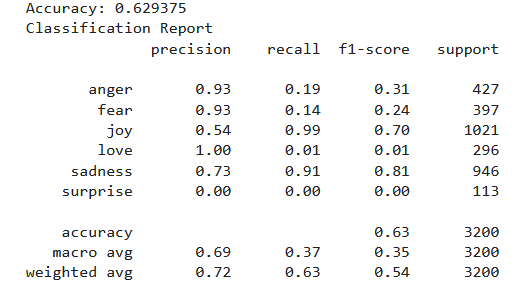
\includegraphics[width=0.8\textwidth]{images/init_result_naive_bayes.png}
	\caption{Naive Bayes Classification Report}
	\label{fig:initial_naive_bayes}
\end{figure}

\begin{figure}[h!]
	\centering
	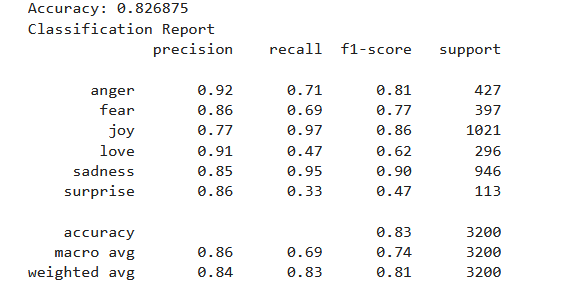
\includegraphics[width=0.8\textwidth]{images/init_result_logistic_regression.png}
	\caption{Logistic Regression Classification Report}
	\label{fig:initial_logistic_regression}
\end{figure}

\begin{figure}[h!]
	\centering
	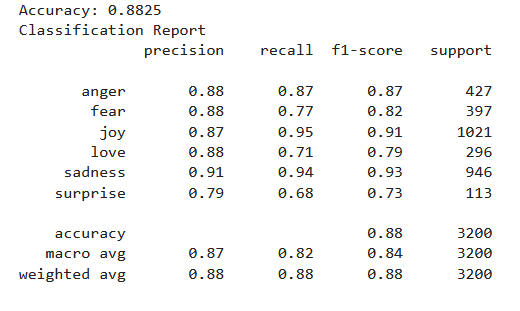
\includegraphics[width=0.8\textwidth]{images/init_result_random_forest.png}
	\caption{Random Forest Classification Report}
	\label{fig:initial_random_forest}
\end{figure}

\begin{figure}[h!]
	\centering
	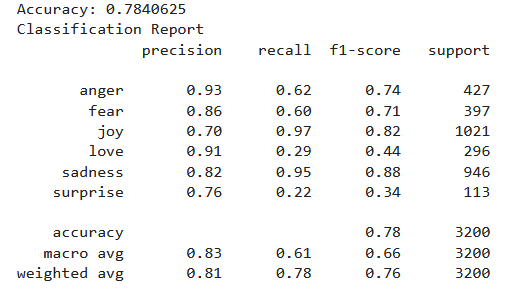
\includegraphics[width=0.8\textwidth]{images/init_result_svm.png}
	\caption{SVM Classification Report}
	\label{fig:initial_svm}
\end{figure}

\begin{figure}[h!]
	\centering
	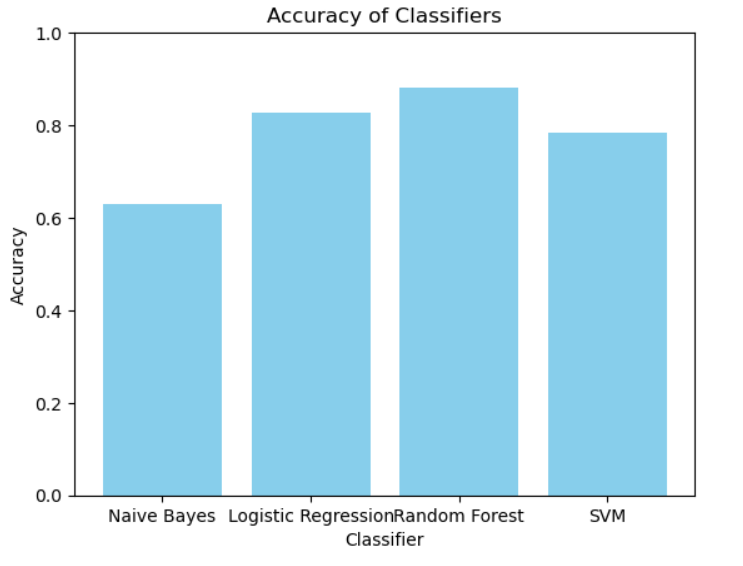
\includegraphics[width=0.8\textwidth]{images/accuracy_model_init_result.png}
	\caption{Initial Accuracy Model}
	\label{fig:initial_accuracy_model}
\end{figure}

\begin{figure}[h!]
	\centering
	% First row
	\begin{subfigure}[b]{0.45\textwidth}
		\centering
		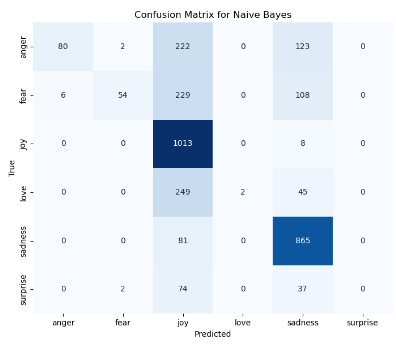
\includegraphics[width=\textwidth]{images/confusion_naive_bayes_init.png}
		\caption{Confusion Matrix for Naive Bayes}
		\label{fig:init_confusion_matrix_naive_bayes}
	\end{subfigure}
	\hfill
	\begin{subfigure}[b]{0.45\textwidth}
		\centering
		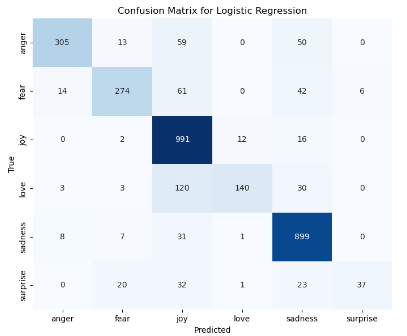
\includegraphics[width=\textwidth]{images/confusion_logistic_regression_init.png}
		\caption{Confusion Matrix for Logistic Regression}
		\label{fig:init_confusion_matrix_logistic_regression}
	\end{subfigure}
	
	% Second row
	\vskip\baselineskip
	\begin{subfigure}[b]{0.45\textwidth}
		\centering
		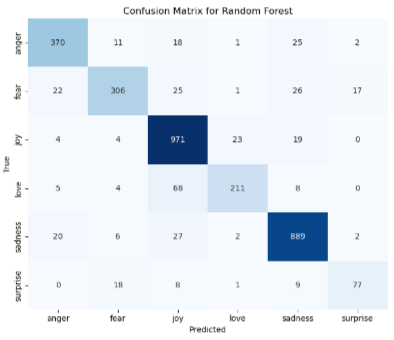
\includegraphics[width=\textwidth]{images/confusion_random_forest_init.png}
		\caption{Confusion Matrix for Random Forest}
		\label{fig:init_confusion_matrix_random_forest}
	\end{subfigure}
	\hfill
	\begin{subfigure}[b]{0.45\textwidth}
		\centering
		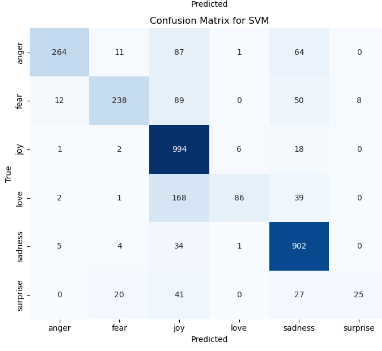
\includegraphics[width=\textwidth]{images/confusion_svm_init.png}
		\caption{Confusion Matrix for SVM}
		\label{init_confusion_matrix_svm}
	\end{subfigure}
	
	\caption{Initial Results Confusion Matrix}
	\label{fig:initial_confusion_matrix}
\end{figure}

\clearpage

\subsection{Naive Bayes}
The Naive Bayes model achieved an accuracy of 0.63 in Figure \ref{fig:initial_naive_bayes}. It demonstrated strong performance in recognizing Joy and Sadness with high recall values for these classes. Notably, the recall for Joy was 0.99, indicating that nearly all joyful instances were correctly identified. However, the model struggled significantly with other emotions such as Anger, Fear, Love, and particularly Surprise where the recall was extremely low at 0.00. This suggests that Naive Bayes had difficulty distinguishing between more nuanced emotions. The F1-scores were moderate for Joy (0.70) and Sadness (0.81), but very low for other categories, indicating poor balance between precision and recall. The confusion matrix showed that Naive Bayes experienced the most misclassifications, particularly between Joy and other emotions like Anger and Fear in Figure \ref{fig:init_confusion_matrix_naive_bayes}."

\subsection{Logistic Regression}
Logistic Regression significantly improved accuracy to 0.83, demonstrating strong performance across most emotions in Figure \ref{fig:initial_logistic_regression}. The model was especially effective in identifying Joy (F1-score: 0.86) and Sadness (F1-score: 0.90), with high recall values of 0.97 and 0.95, respectively, indicating reliable identification of these emotions. It also performed well for Anger and Fear with good precision and recall metrics. However, the emotions Love and Surprise showed slightly lower recall values of 0.47 and 0.33, respectively, suggesting that these emotions were harder to predict accurately. While Logistic Regression reduced misclassifications overall, "love" and "surprise" remained challenging for the model.

\subsection{Random Forest}
The Random Forest model achieved the highest accuracy at 0.88, outperforming both Logistic Regression and Naive Bayes in Figure \ref{fig:initial_random_forest}. It performed very well on Joy, Sadness, Fear, and Anger, with F1-scores around or exceeding 0.80. While the recall for Love and Surprise was still lower at 0.79 and 0.73, respectively, this was an improvement over the other models. Random Forest showed a balanced performance between precision and recall across most emotion categories, making it the best performer overall in this context. This model's ability to maintain high scores for harder-to-classify emotions like Love and Surprise highlighted its robustness.

\subsection{Support Vector Machine (SVM)}
The SVM model achieved an accuracy of 0.85, performing comparably to Logistic Regression. It exhibited strong precision and recall for Anger, Fear, Joy, and Sadness in Figure \ref{fig:initial_svm}" However, similar to Logistic Regression, Love and Surprise had lower recall values of 0.29 and 0.22, respectively, suggesting these emotions posed a challenge for the model. Despite these challenges, SVM achieved strong F1-scores for major emotion categories such as Joy (0.82) and Sadness (0.88). While its overall performance was commendable, SVM also faced difficulties with Love and Surprise, similar to other models.

\subsection{Overall Insights for Initial Results}
The Random Forest model emerged as the best-performing model, achieving the highest accuracy (88.25\%) and demonstrating a well-balanced performance across most emotions. However, all models faced challenges with Love and Surprise, which showed lower recall and F1-scores. These difficulties could be attributed to the lower frequency of these emotions in the dataset or their nuanced nature. The Naive Bayes model, while effective for simpler tasks, struggled significantly with complex emotions and exhibited poor performance on less common categories like Surprise and Love. This analysis underscores the importance of using more robust models like Random Forest for achieving better balance and accuracy in emotion classification tasks.

       
\subsection{Final Results}
The following are the precision, recall, F1-score, and support metrics for each classification model, evaluating its performance across six emotion categories: Sadness, Joy, Love, Anger, Fear, and Surprise.

\begin{figure}[h!]
\centering
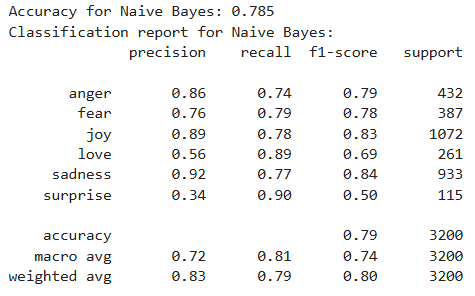
\includegraphics[width=0.8\textwidth]{images/naive_bayes_result.png}
\caption{Naive Bayes Classification Report}
\label{fig:naive_bayes}
\end{figure}

\begin{figure}[h!]
\centering
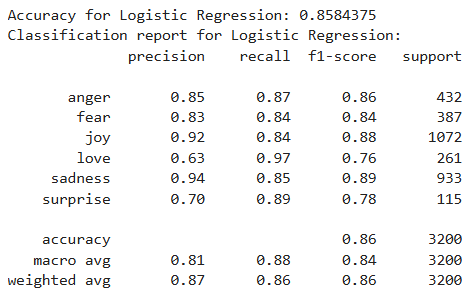
\includegraphics[width=0.8\textwidth]{images/logistic_regression_result.png}
\caption{Logistic Regression Classification Report}
\label{fig:logistic_regression}
\end{figure}

\begin{figure}[h!]
\centering
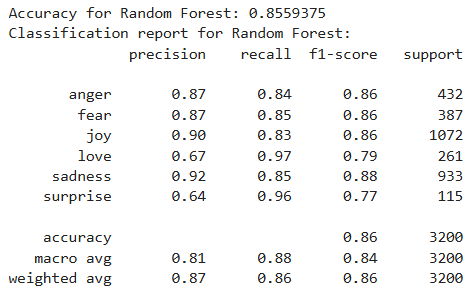
\includegraphics[width=0.8\textwidth]{images/random_forest_result.png}
\caption{Random Forest Classification Report}
\label{fig:random_forest}
\end{figure}

\begin{figure}[h!]
\centering
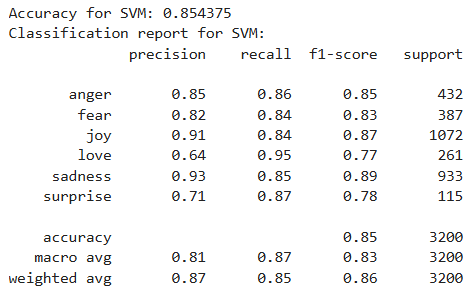
\includegraphics[width=0.8\textwidth]{images/svm_result.png}
\caption{SVM Classification Report}
\label{fig:svm}
\end{figure}

\begin{figure}[h!]
\centering
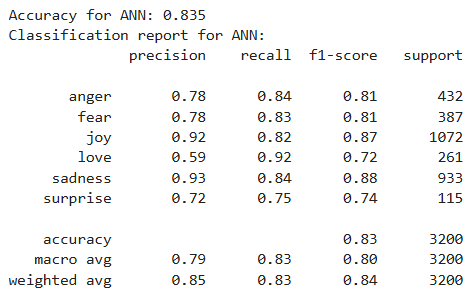
\includegraphics[width=0.8\textwidth]{images/ann_result.png}
\caption{ANN Classification Report}
\label{fig:ann}
\end{figure}

\begin{figure}[h!]
\centering
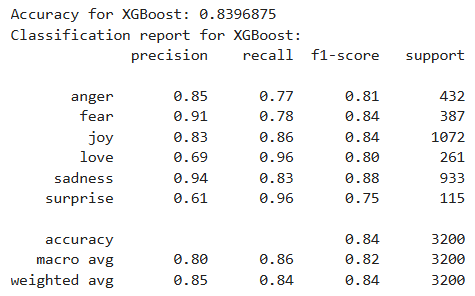
\includegraphics[width=0.8\textwidth]{images/xgboost_result.png}
\caption{XGBoost Classification Report}
\label{fig:xgboost}
\end{figure}

\clearpage

\subsection{Naive Bayes Result}
The Naive Bayes model achieved an accuracy of 0.785. It performed reasonably well across several emotions, with Sadness showing the highest recall (0.77) and Surprise the lowest precision (0.34) as shown in Figure \ref{fig:naive_bayes}. The weighted average F1-score of 0.80 indicates balanced performance across emotions, though some areas like Surprise and Love could be improved. In terms of precision, the model had the best result for Sadness (0.92).

\subsection{Logistic Regression Result}
Logistic Regression showed the highest accuracy at 0.8584, as displayed in Figure \ref{fig:logistic_regression}. It achieved solid F1-scores across emotions, with Sadness and Joy showing excellent results (F1-scores of 0.89 and 0.88, respectively). The model performed particularly well in Love with a precision of 0.63 and recall of 0.97, which led to a high F1-score of 0.76. The overall weighted average F1-score of 0.86 reflects its strong performance, particularly in Anger, Joy, and Sadness.

\subsection{Random Forest Result}
The Random Forest model delivered an accuracy of 0.8559, close to that of Logistic Regression, as shown in Figure \ref{fig:random_forest}. The model showed good precision and recall across emotions, with Sadness again being a strong performer (precision 0.92, recall 0.85). Notably, Love and Surprise had slightly lower precision scores, though the weighted average F1-score of 0.86 suggests robust performance overall, with good consistency between precision and recall.

\subsection{Support Vector Machine (SVM) Result}
SVM achieved an accuracy of 0.8544, performing similarly to Random Forest, as depicted in Figure \ref{fig:svm}. The Anger class had a precision of 0.85 and recall of 0.86, contributing to a high F1-score. Surprise had relatively high precision (0.71) and recall (0.87), leading to a balanced F1-score. This indicates SVM's ability to generalize well, even with some misclassifications in less frequent emotions like Surprise.

\subsection{Artificial Neural Network (ANN) Result}
ANN had an accuracy of 0.835, which was the lowest among the models tested, as shown in Figure \ref{fig:ann}. Despite this, it achieved impressive recall in Love (0.92), showing its strength in detecting emotional subtleties in such cases. However, it struggled with Surprise, as reflected in the F1-score of 0.74. The overall macro average F1-score of 0.80 highlights ANN's potential, although it might need additional tuning to improve accuracy across all emotions.

\subsection{XGBoost Result}
XGBoost showed an accuracy of 0.8397 and demonstrated good overall performance, particularly with Fear (precision 0.91, recall 0.78), as shown in Figure \ref{fig:xgboost}. The model performed reasonably well with Sadness and Love, achieving balanced results in both precision and recall. However, Surprise showed lower precision (0.61), impacting the F1-score, which was still relatively high at 0.75. The overall model's weighted F1-score of 0.84 indicates a solid all-around performance.

\subsection{Model Accuracy Comparison}
\begin{figure}[h!]
\centering
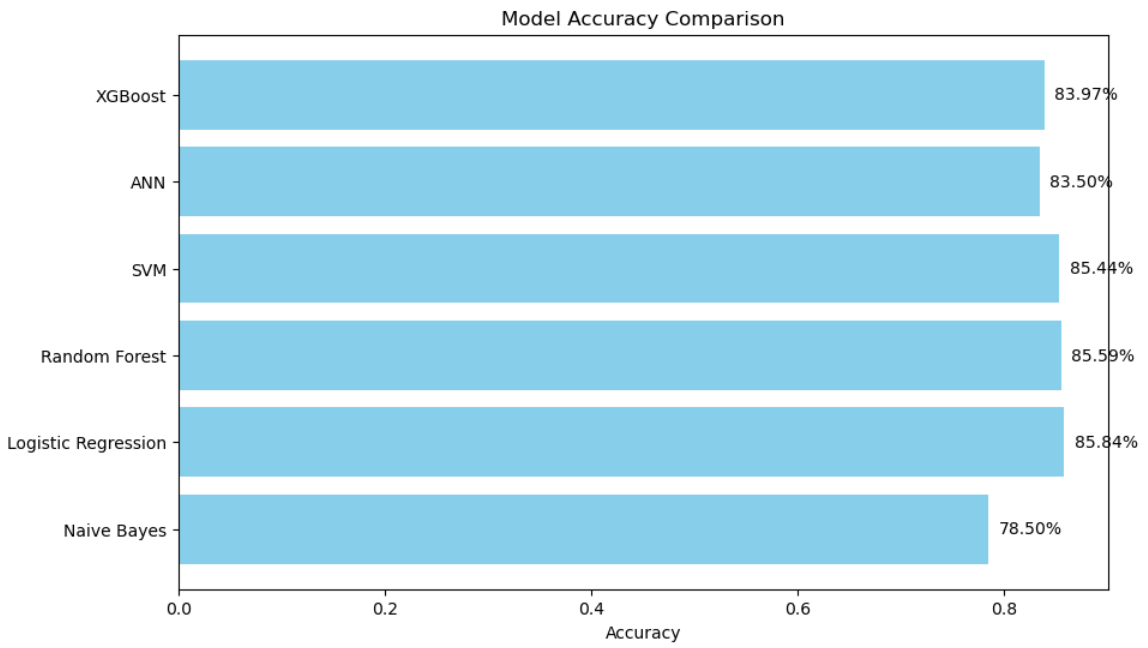
\includegraphics[width=0.8\textwidth]{images/model_accuracy.png}
\caption{Model Accuracy Comparison}
\label{fig:model_accuracy}
\end{figure}

As shown in Figure \ref{fig:model_accuracy}, Logistic Regression emerged as the top-performing model with an accuracy of \textbf{0.8584}. It was closely followed by Random Forest (\textbf{0.8559}) and SVM (\textbf{0.8544}). ANN achieved the lowest accuracy at \textbf{0.835}, highlighting the potential for further improvements in performance. XGBoost showed a solid accuracy of \textbf{0.8397}, rounding out the list of top models.

Logistic Regression performed exceptionally well across all emotion categories, with Random Forest and SVM also demonstrating strong results. Although ANN had the lowest accuracy, its strong recall in detecting emotions such as Love suggests it could be improved with further tuning. XGBoost demonstrated competitive performance but could benefit from addressing lower precision in emotions like Surprise. The results indicate that further optimization of hyperparameters for each model could enhance their performance, especially for less represented emotions.

\clearpage


% CONFUSION MATRICES

\subsection{Confusion Matrices}

\begin{figure}[h!]
	\centering
	% First row
	\begin{subfigure}[b]{0.45\textwidth}
		\centering
		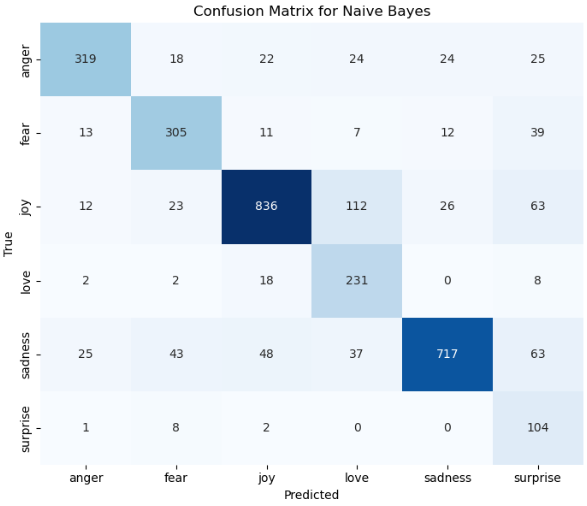
\includegraphics[width=\textwidth]{images/confusion_matrix_01.png}
		\caption{Confusion Matrix for Naive Bayes}
		\label{fig:final_confusion_matrix_naive_bayes}
	\end{subfigure}
	\hfill
	\begin{subfigure}[b]{0.45\textwidth}
		\centering
		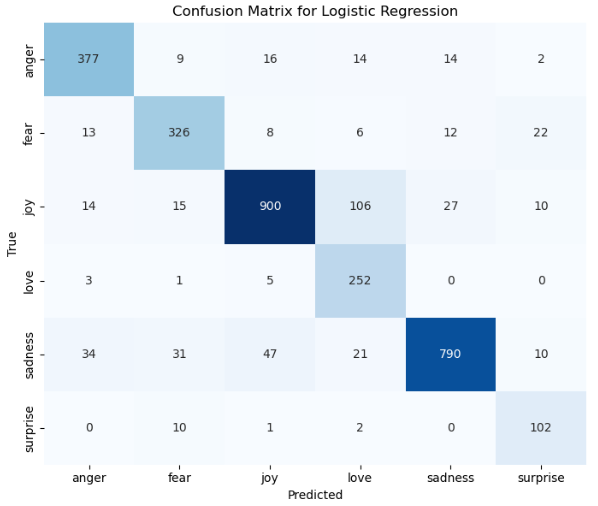
\includegraphics[width=\textwidth]{images/confusion_matrix_01.1.png}
		\caption{Confusion Matrix for Logistic Regression}
		\label{fig:final_confusion_matrix_logistic_regression}
	\end{subfigure}
	
	% Second row
	\vskip\baselineskip
	\begin{subfigure}[b]{0.45\textwidth}
		\centering
		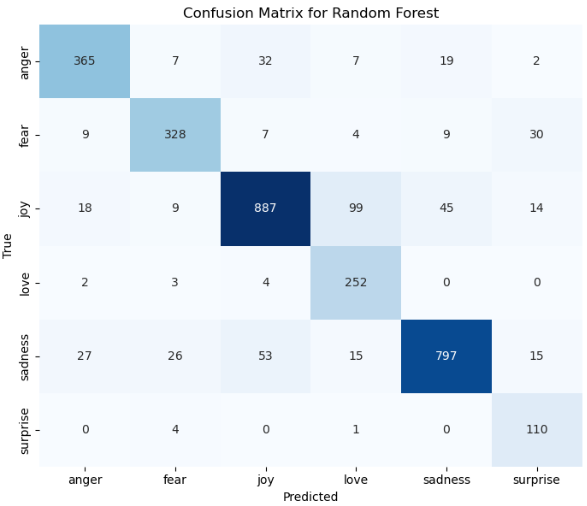
\includegraphics[width=\textwidth]{images/confusion_matrix_02.png}
		\caption{Confusion Matrix for Random Forest}
		\label{fig:final_confusion_matrix_random_forest}
	\end{subfigure}
	\hfill
	\begin{subfigure}[b]{0.45\textwidth}
		\centering
		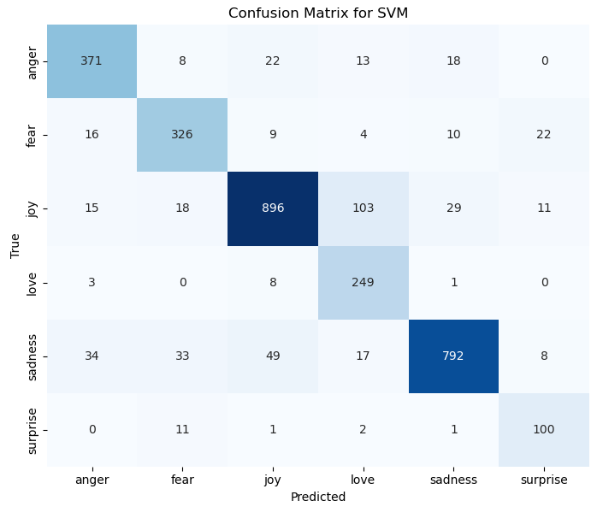
\includegraphics[width=\textwidth]{images/confusion_matrix_02.1.png}
		\caption{Confusion Matrix for SVM}
		\label{fig:final_confusion_matrix_svm}
	\end{subfigure}
	
	% Third row
	\vskip\baselineskip
	\begin{subfigure}[b]{0.45\textwidth}
		\centering
		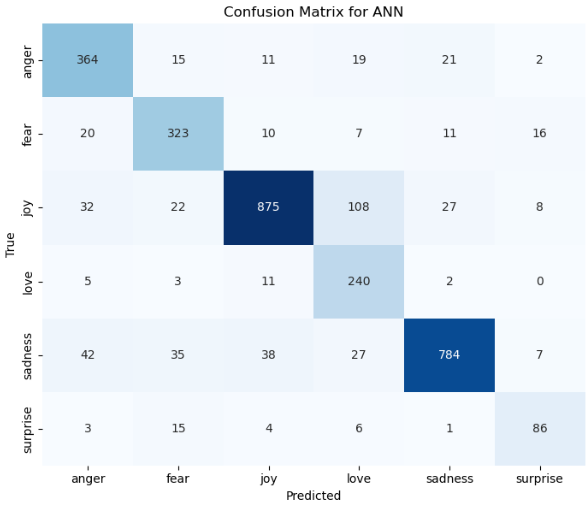
\includegraphics[width=\textwidth]{images/confusion_matrix_03.png}
		\caption{Confusion Matrix for ANN}
		\label{fig:final_confusion_matrix_ann}
	\end{subfigure}
	\hfill
	\begin{subfigure}[b]{0.45\textwidth}
		\centering
		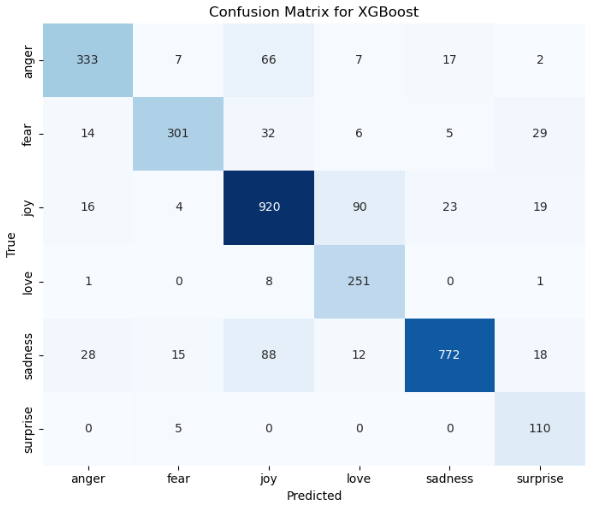
\includegraphics[width=\textwidth]{images/confusion_matrix_03.1.png}
		\caption{Confusion Matrix for XGBoost}
		\label{fig:final_confusion_matrix_xgboost}
	\end{subfigure}
	
	
	\caption{Final Results Confusion Matrix}
	\label{fig:final_confusion_matrix}
\end{figure}

The confusion matrices for each model show significant improvements in true positive results after applying optimizations. Among all emotion categories, Joy consistently achieves the highest true positive counts across all models, followed by Sadness. These results suggest that the models are particularly effective at identifying these two emotions, likely due to their distinct features and higher frequency in the dataset.

There is a notable improvement in the new results compared to the previous ones, where the true positive counts for some categories, such as Love and Surprise were effectively zero. While these values remain low, they have significantly improved. For instance, Naive Bayes previously had zero true positive counts for Love and Surprise. After the distribution modifications, these values increased to 231 and 104, respectively. The fact that they are no longer zero indicates that the applied optimizations, such as stratified sampling and hyperparameter tuning, had a meaningful impact, even on the weakest-performing model.

For the other models, the improvements are also evident in the previously challenging categories of Love and Surprise. After optimization, these models now demonstrate significantly higher true positive counts for these emotions. Love has achieved a true positive count of around 200 in most models, while Surprise has improved to approximately 80 to 100. Despite these gains, ANN has the lowest true positive count for Surprise, with only 88, indicating it still struggles with this emotion. On the other hand, Random Forest demonstrates exceptional performance for Love and Surprise, achieving a true positive count of 252 and 110 respectively, the highest among all models.

These results highlight the effectiveness of the optimizations in addressing imbalanced and nuanced emotion categories while underscoring the strengths and limitations of each model.

\clearpage

% METRICS

\begin{figure}[h!]
	\centering
	% First row
	\begin{subfigure}[b]{0.45\textwidth}
		\centering
		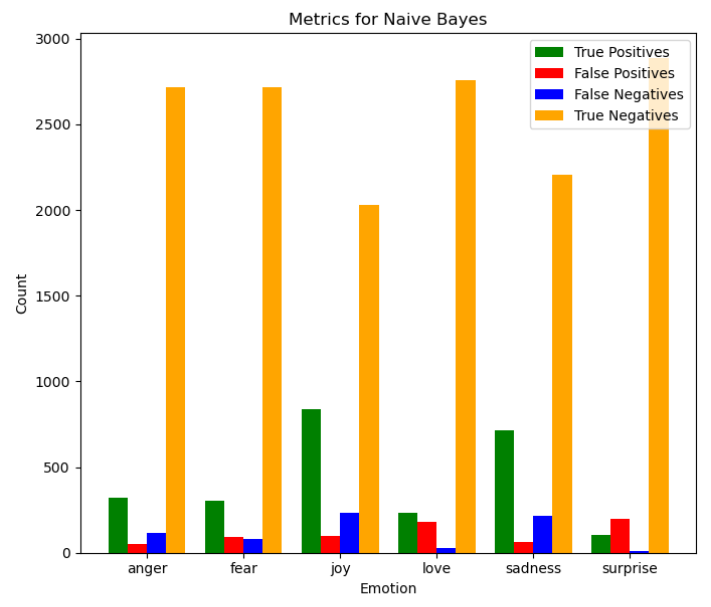
\includegraphics[width=\textwidth]{images/metrics_naive_bayes.png}
		\caption{Metrics for Naive Bayes}
		\label{fig:metrics_evaluation_naive_bayes}
	\end{subfigure}
	\hfill
	\begin{subfigure}[b]{0.45\textwidth}
		\centering
		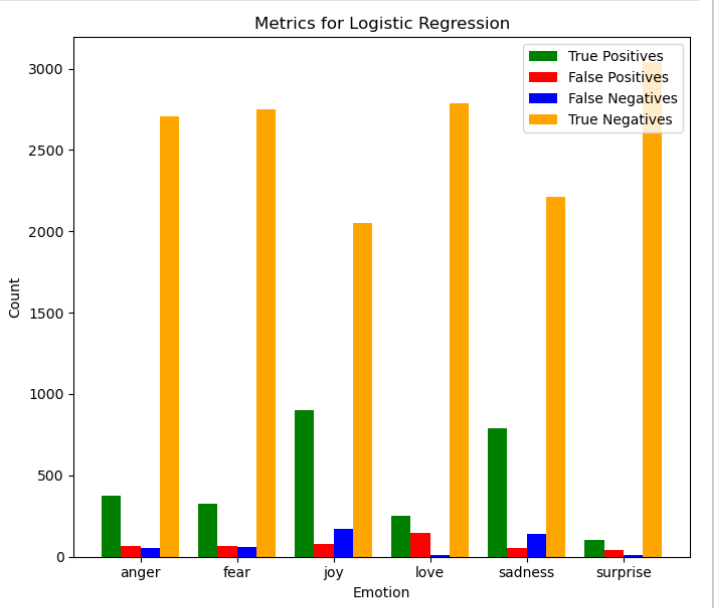
\includegraphics[width=\textwidth]{images/metrics_logistic_regression.png}
		\caption{Metrics for Logistic Regression}
		\label{fig:metrics_evaluation_logistic_regression}
	\end{subfigure}
	
	% Second row
	\vskip\baselineskip
	\begin{subfigure}[b]{0.45\textwidth}
		\centering
		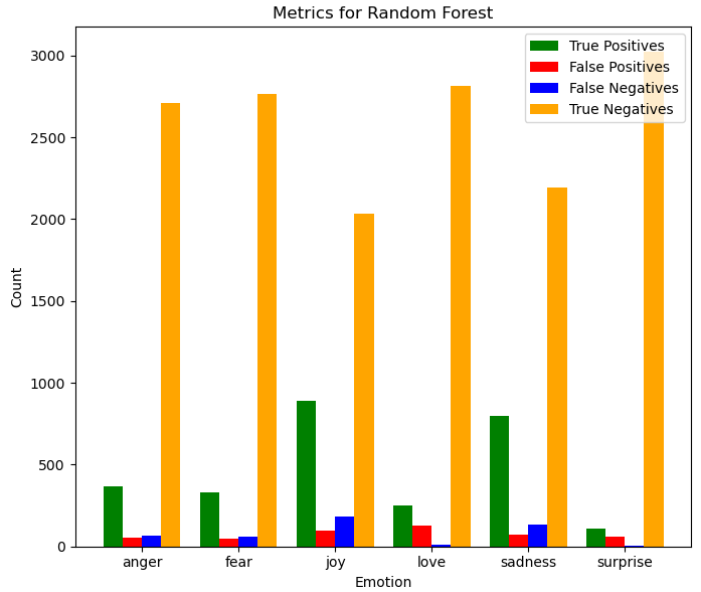
\includegraphics[width=\textwidth]{images/metrics_random_forest.png}
		\caption{Metrics for Random Forest}
		\label{fig:metrics_evaluation_random_forest}
	\end{subfigure}
	\hfill
	\begin{subfigure}[b]{0.45\textwidth}
		\centering
		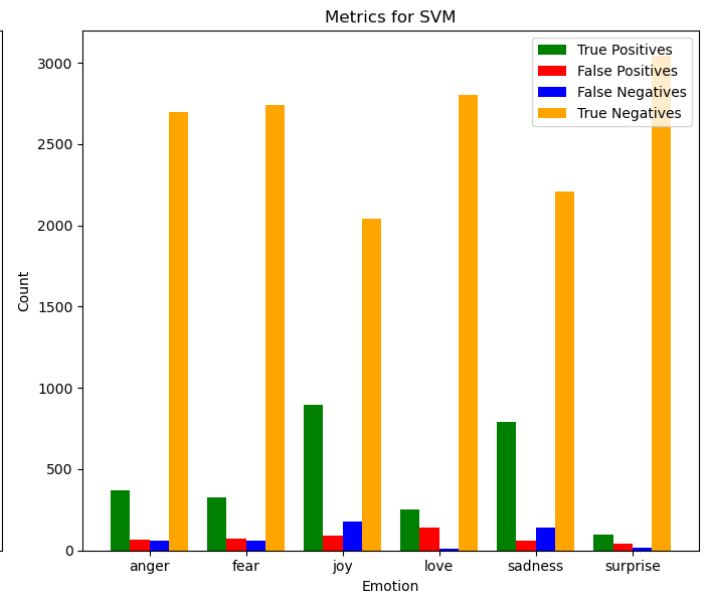
\includegraphics[width=\textwidth]{images/metrics_svm.png}
		\caption{Metrics for SVM}
		\label{fig:metrics_evaluation_svm}
	\end{subfigure}
	
	% Third row
	\vskip\baselineskip
	\begin{subfigure}[b]{0.45\textwidth}
		\centering
		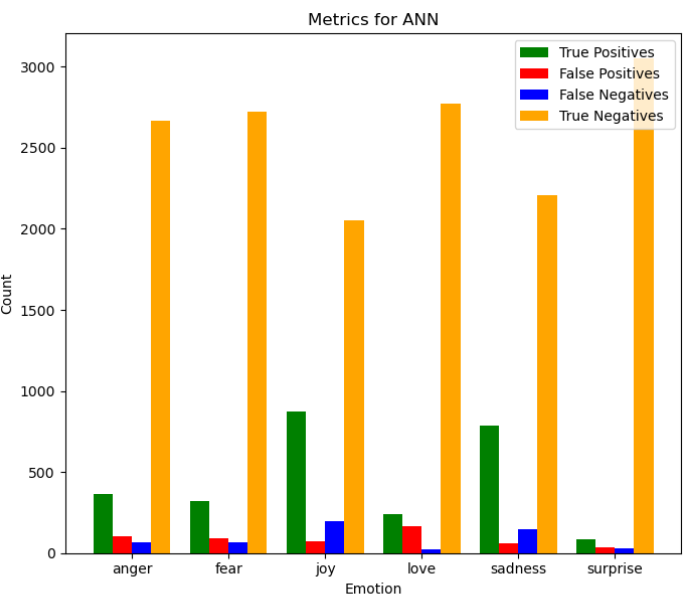
\includegraphics[width=\textwidth]{images/metrics_ann.png}
		\caption{Metrics for ANN}
		\label{fig:metrics_evaluation_matrix_ann}
	\end{subfigure}
	\hfill
	\begin{subfigure}[b]{0.45\textwidth}
		\centering
		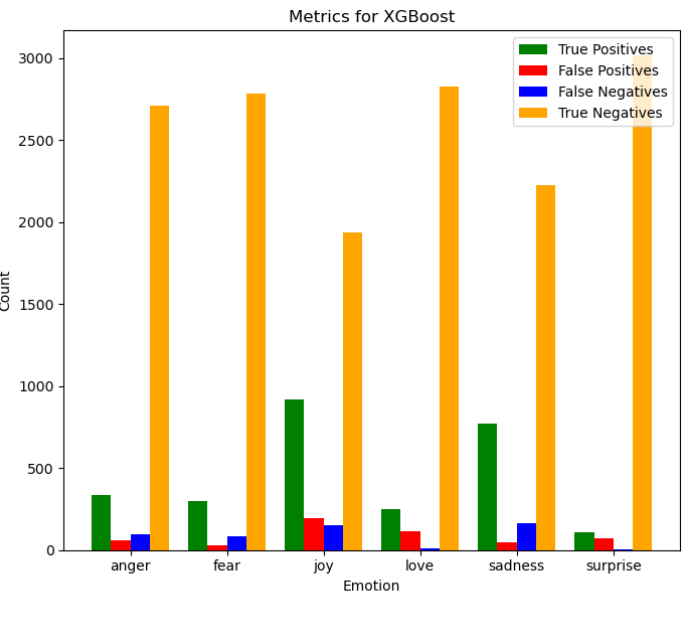
\includegraphics[width=\textwidth]{images/metrics_xgboost.png}
		\caption{Metrics for XGBoost}
		\label{fig:metrics_evaluation_xgboost}
	\end{subfigure}
	
	
	\caption{Metrics for Models}
	\label{fig:metrics_evaluation}
\end{figure}

For the metrics evaluation across all models in Figure \ref{fig:metrics_evaluation}, Surprise consistently exhibits the highest number of True Negatives, followed by Love, Fear, and Anger. On the other hand, Joy achieves the highest True Positive count, closely followed by Sadness. The distribution of False Positives and False Negatives varies across the models, highlighting differences in their misclassification patterns. These trends indicate that while some emotions are more easily distinguished by the models, others, like Surprise and Love, may still pose challenges, depending on the specific classification algorithm.

The bar chart visualizing the confusion matrix metrics for the Random Forest model further reveals these trends. True Positives (TP), False Positives (FP), False Negatives (FN), and True Negatives (TN) are displayed for each emotion class. True Negatives (TN) dominate across most emotions, which suggests that the model is very good at correctly identifying the absence of certain emotions. 

\begin{itemize}
    \item \textbf{True Positives (Green):} These indicate the number of times the model correctly predicted a given emotion. Emotions like Joy and Sadness have relatively higher TPs, signaling better performance for these classes.
    \item \textbf{False Positives (Red):} These represent cases where the model predicted an emotion that wasn’t actually present. For emotions such as Fear and Joy, FP instances are comparatively low, meaning fewer misclassifications.
    \item \textbf{False Negatives (Blue):} Instances where the model failed to predict the emotion when it was actually present. For some classes, such as Anger and Love, FN is relatively higher, suggesting that the model struggles to detect these emotions.
    \item \textbf{True Negatives (Orange):} TN values are significantly high for all emotions, indicating that the model performs well in avoiding false alarms for these emotion classes.
\end{itemize}

\clearpage

% RO CURVE

\begin{figure}[h!]
	\centering
	% First row
	\begin{subfigure}[b]{0.45\textwidth}
		\centering
		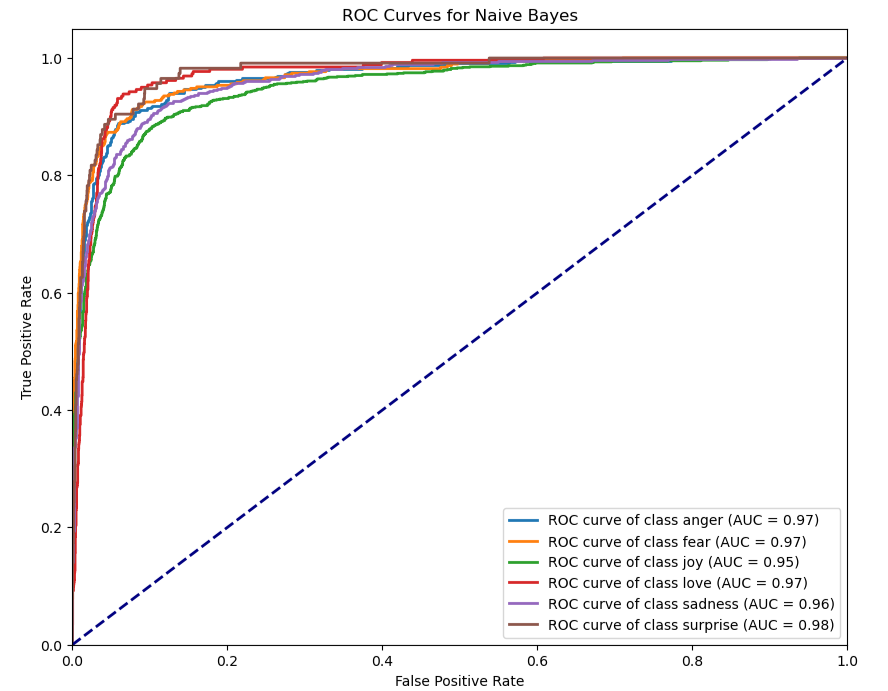
\includegraphics[width=\textwidth]{images/roc_naive_bayes.png}
		\caption{ROC for Naive Bayes}
		\label{fig:roc_naive_bayes}
	\end{subfigure}
	\hfill
	\begin{subfigure}[b]{0.45\textwidth}
		\centering
		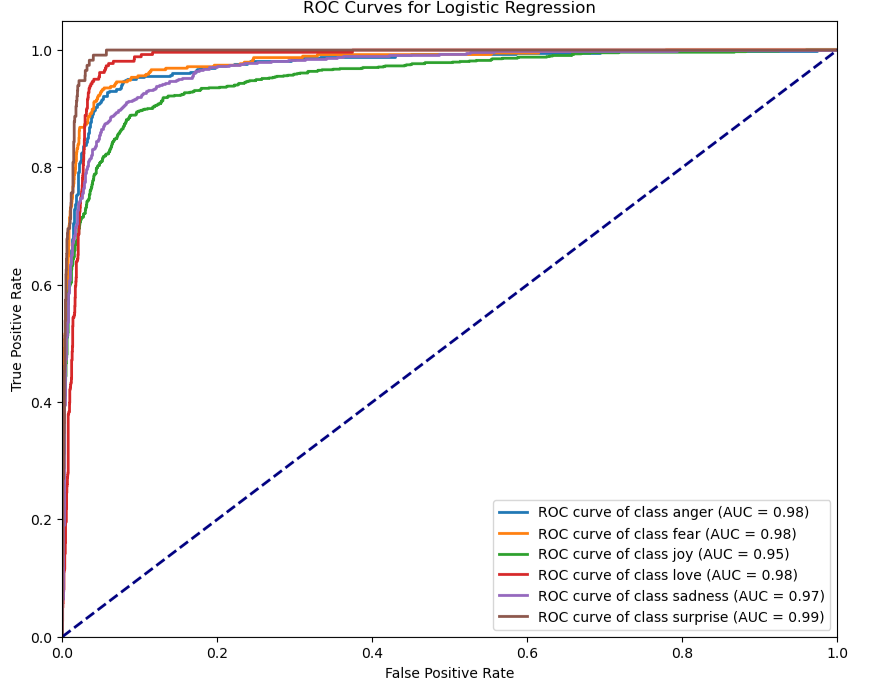
\includegraphics[width=\textwidth]{images/roc_logistic_regression.png}
		\caption{ROC for Logistic Regression}
		\label{fig:roc_logistic_regression}
	\end{subfigure}
	
	% Second row
	\vskip\baselineskip
	\begin{subfigure}[b]{0.45\textwidth}
		\centering
		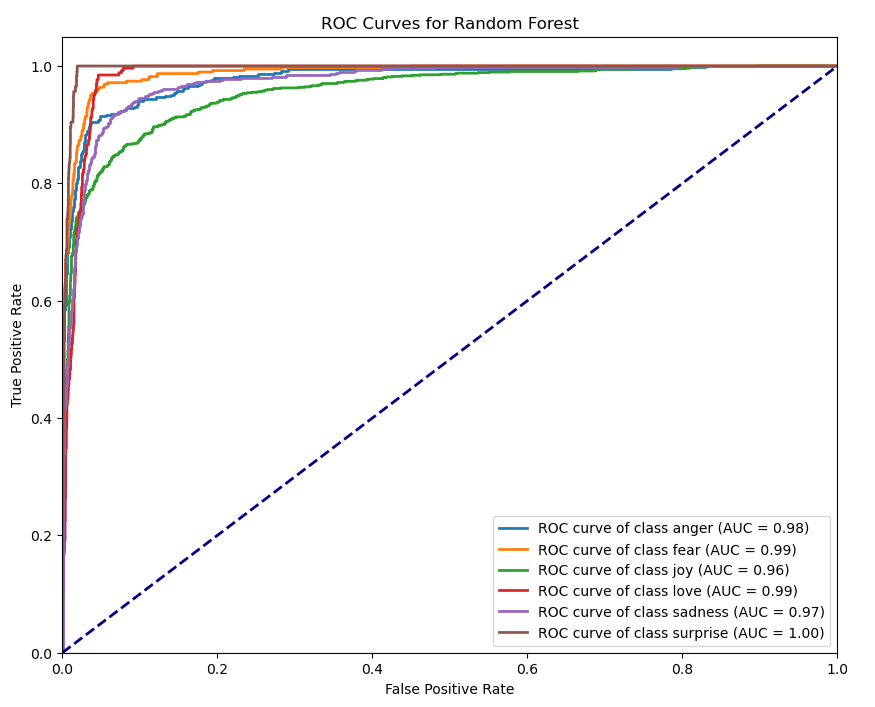
\includegraphics[width=\textwidth]{images/roc_random_forest.png}
		\caption{ROC for Random Forest}
		\label{fig:roc_forest}
	\end{subfigure}
	\hfill
	\begin{subfigure}[b]{0.45\textwidth}
		\centering
		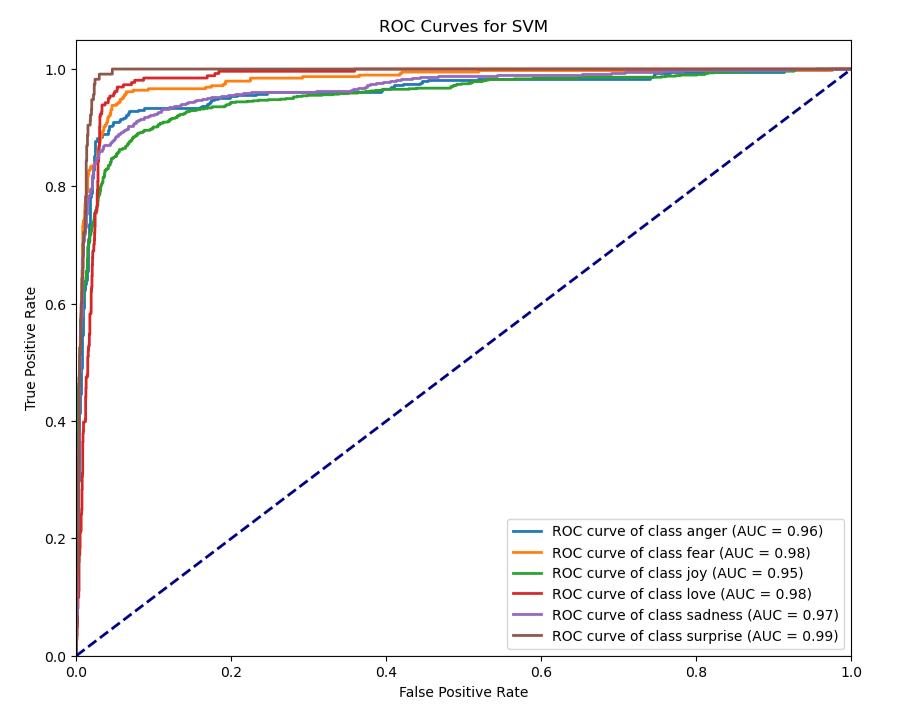
\includegraphics[width=\textwidth]{images/roc_svm.png}
		\caption{ROC for SVM}
		\label{fig:roc_svm}
	\end{subfigure}
	
	% Third row
	\vskip\baselineskip
	\begin{subfigure}[b]{0.45\textwidth}
		\centering
		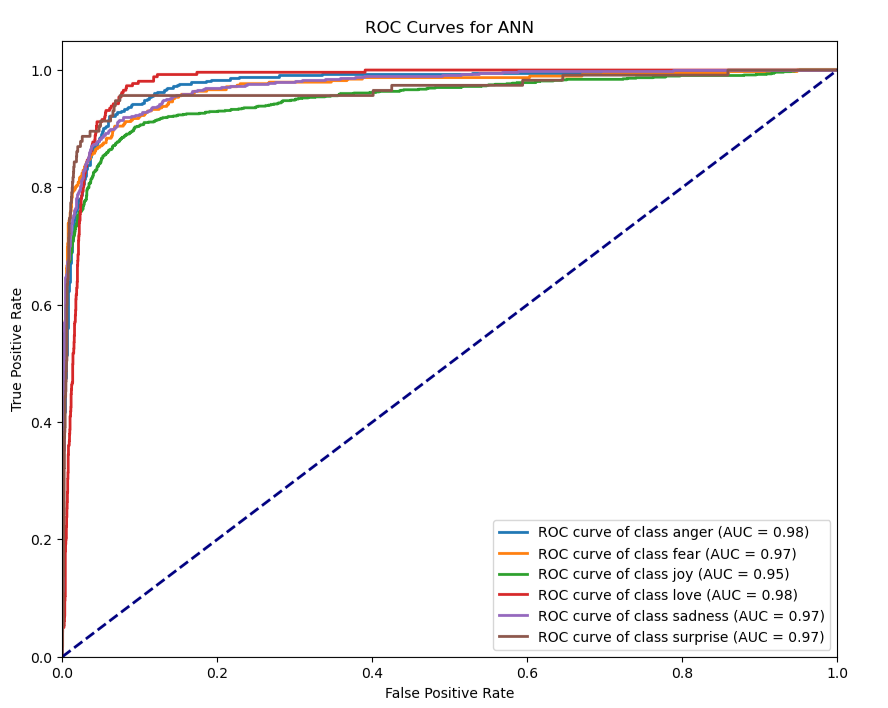
\includegraphics[width=\textwidth]{images/roc_ann.png}
		\caption{ROC for ANN}
		\label{fig:roc_ann}
	\end{subfigure}
	\hfill
	\begin{subfigure}[b]{0.45\textwidth}
		\centering
		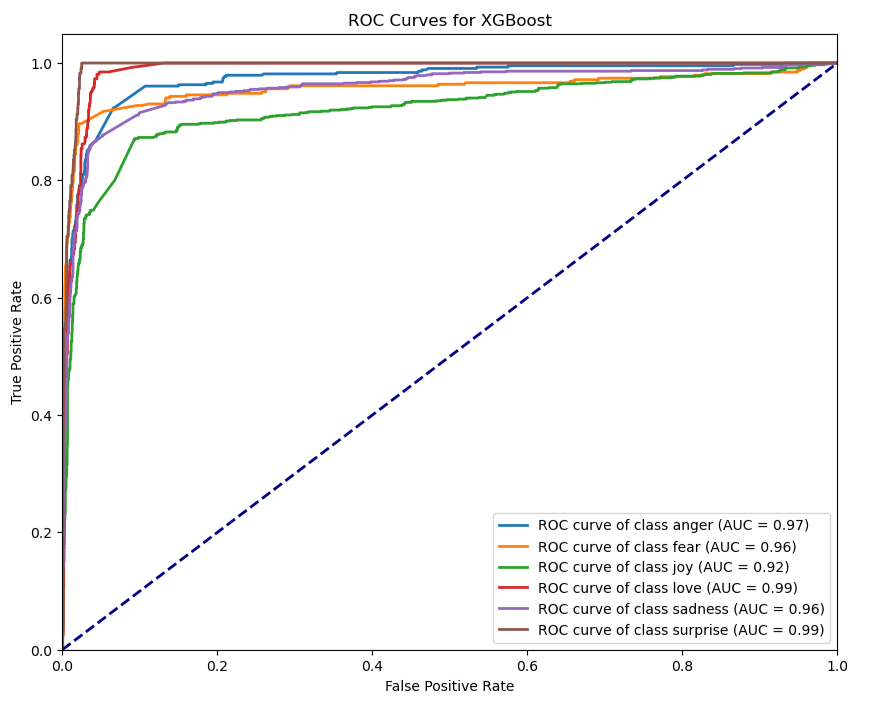
\includegraphics[width=\textwidth]{images/roc_xgboost.png}
		\caption{ROC for XGBoost}
		\label{fig:roc_xgboost}
	\end{subfigure}
	
	
	\caption{RO Curve for Models}
	\label{fig:roc}
\end{figure}

The ROC curves for the models show a high degree of classification performance across all emotion categories, as indicated by the Area Under the Curve (AUC) values. Random Forest demonstrate an AUC of 1.00 for Surprise and consistently high scores across all categories, indicating excellent discrimination. However, since an AUC of 1.00 is rare in practice, it might indicate potential overfitting, data leakage, or unusually strong signals in the dataset for this specific class. Similarly, SVM achieves near-perfect AUC values for Fear, Love, and Surprise.

Naive Bayes, while generally lower in classification accuracy compared to other models, shows respectable AUC values ranging from 0.95 to 0.98, indicating improved ability to separate classes after optimization. Logistic Regression and ANN also perform well, with AUC values typically above 0.95, showcasing their robustness in emotion detection.

XGBoost shows competitive performance with high AUC values, particularly excelling in Love (AUC = 0.99) and Surprise (AUC = 0.99). However, its AUC for Joy (0.92) is slightly lower compared to other models.

%Overall, Random Forest emerges as the most consistent and reliable model, especially for harredict classes like "Surprise," while other models also display strong discrimination ability, as reflected by their high AUC values.

\clearpage